\documentclass[12pt]{report}
\usepackage{graphicx}
\usepackage{amsmath}
\usepackage{parskip}
\usepackage{wrapfig}
\usepackage{subcaption}
\usepackage{float}
\graphicspath{ {./images/} }

\title{{Progetto di Meccatronica}\\{Robotic sorter}}

\author{{Tosi Ubaldo}\\{Passerella Filippo}}

\begin{document}
\maketitle

\tableofcontents

\chapter{Introduzione}

Abbiamo realizzato il controllo di un manipolatore per smistamento di cubi colorati.

Il sistema riconosce il colore del cubo posto sull'apposita pedana e lo riposiziona nella zona appropriata. Poi torna alla posizione iniziale, in attesa del cubo seguente.

Abbiamo provato il sistema in più condizioni e non ci sono noti casi di malfunzionamento in ambiente adatto.

\section{Divisione delle funzioni}

Abbiamo deciso di dividere il programma finale in due parti, un modulo di percezione e un modulo di attuazione.

\begin{figure}
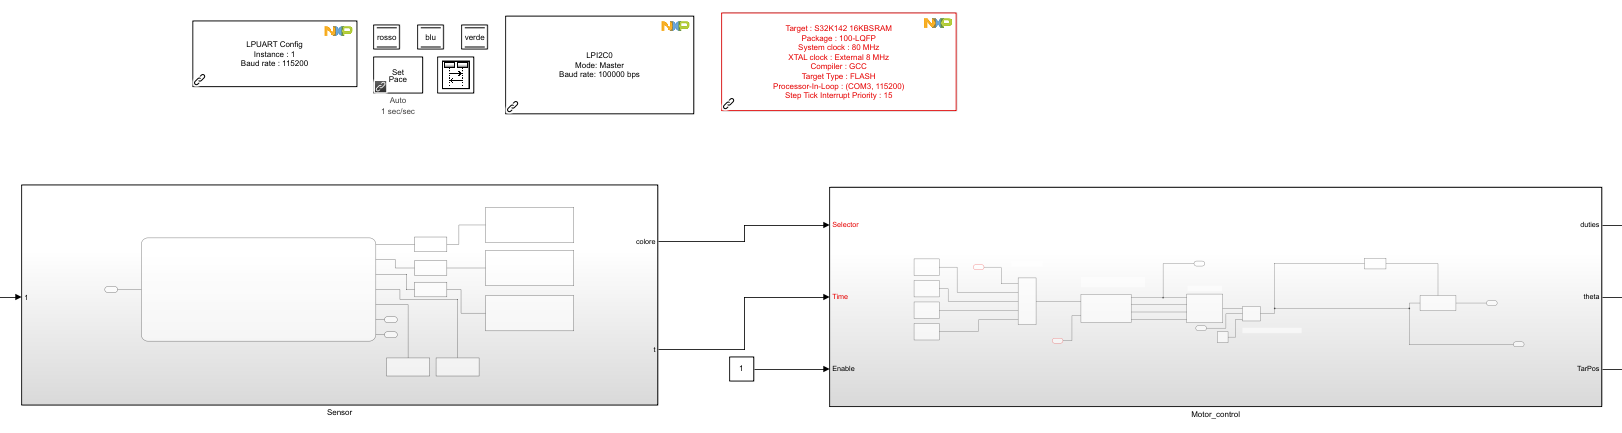
\includegraphics[width=\textwidth]{Modules}
\caption{Moduli}
\end{figure}

Il primo si occupa di interfacciarsi con il sensore di colore e temporizzare il secondo. Il secondo controlla il manipolatore e gestisce i percorsi.

Le funzioni dei due moduli erano sufficientemente indipendenti da poter essere sviluppati e verificati parallelamente.

Ottenuti dei prototipi funzionanti dei due moduli, abbiamo definito l'interfaccia che ha poi determinato la loro versione finale.

\section{Modalità d'uso}

Innanzitutto, occorre collegare l'hardware e accendere il dispositivo.

\begin{table}[h]
\centering
\begin{tabular}{|c|c|c|}
    Collegamento & Porta & Pin \\
    I2C SCL & PTA-3 & J1-3 \\
    I2C SDA & PTA-2 & J1-1 \\
    5V sensore &  & J3-9 \\
    GND sensore &  & J3-11 \\
    GND servo &  & J3-13 \\
    PWM M1 & PTB-12 & J4-3 \\
    PWM M2 & PTB-13 & J5-11 \\
    PWM M3 & PTC-2 & J5-15 \\
    PWM M4 & PTC-3 & J4-16 \\
    PWM M5 & PTB-4 & J2-7 \\
    PWM M6 & PTB-5 & J2-5 \\

\end{tabular}
\end{table}

Si vedrà il braccio posizionarsi nella configurazione di attesa.

Posizionare un cubo colorato sulla pedana e premere \emph{sw2}.

Il manipolatore sposterà il cubo nella zona appropriata e tornerà nella configurazione di attesa.

\chapter{Percezione}
\section {Sensore di colore}

\begin{figure}
\centering
    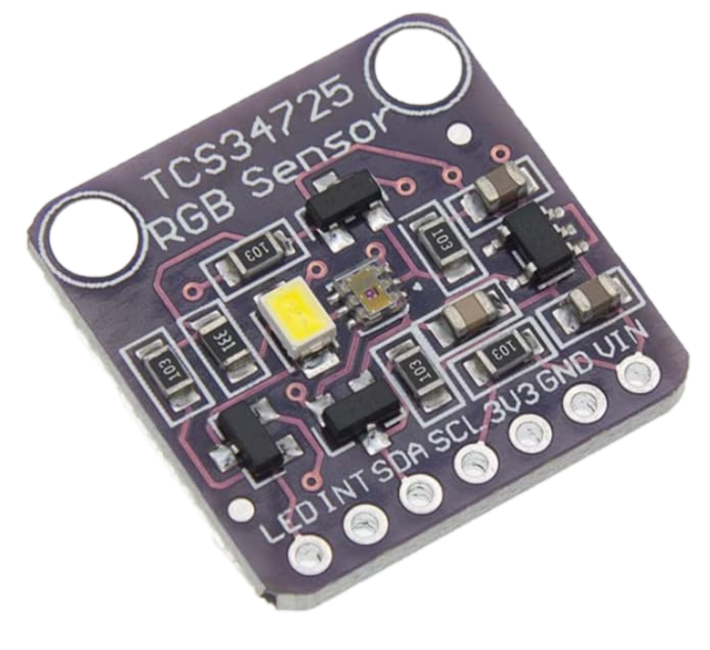
\includegraphics[width=0.4\textwidth]{Immagini_sensore/pcb_sensore.png}
    \caption{PCB Sensore}
\end{figure}

Il PCB del sensore di colore è costituito da

\begin{itemize}
\item il sensore di colore vero e proprio (TAOS TCS3472)
\item un led bianco (che permette di illuminare gli oggetti per misurare il colore della luce riflessa), spegnibile nel caso in cui si voglia misurare il colore di uno schermo o comunque qualcosa che emette luce propria
\item un regolatore $5V \rightarrow 3.3V$, che ci permette di alimentare il sensore a 5V e di usare la I2C a 5V per comunicare con il sensore (grazie a due transistori messi come in figura \ref{fig:I2C})
\item resistenze di pull-up
\end{itemize}

\begin{figure}
\centering
    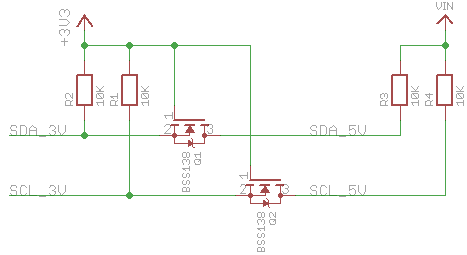
\includegraphics[width=0.4\textwidth]{Immagini_sensore/I2C_3V3_to_5.png}
    \caption{I2C}
    \label{fig:I2C}
\end{figure}

\section{TAOS TCS3472}

\begin{figure}
\centering
    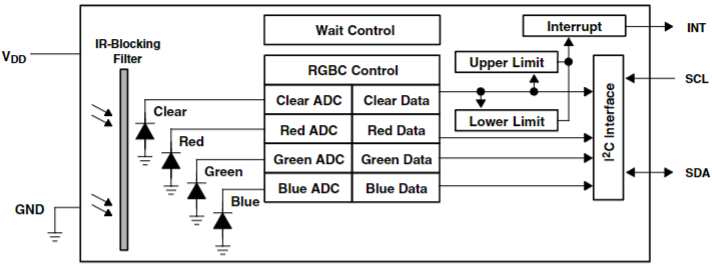
\includegraphics[width=0.4\textwidth]{Immagini_sensore/Blocco_funzionale.png}
    \caption{Blocco funzionale}
\end{figure}
    
\begin{figure}
\centering
    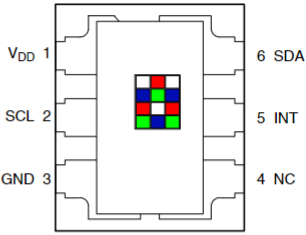
\includegraphics[width=0.4\textwidth]{Immagini_sensore/sensore.png}
    \caption{Matrice fotodiodi sensore}
\end{figure}

Il sensore è costituito da una matrice 3x4 di fotodiodi con un filtro rosso, blu, verde e non filtrati (luce bianca). Tutti i fotodiodi hanno un filtro ad infrarossi per aumentare l'accuratezza. 

La corrente generata da questi fotodiodi viene amplificata da un amplificatore trans-resistivo a guadagno variabile e campionata da un ADC integrativo a 16 bit per ogni colore. Il tempo di integrazione è programmabile. I dati poi vengono comunicati all'esterno attraverso l'interfaccia I2C (fino a 400 KHz).

 Il sensore può mandare un interrupt una volta che il valore del clear è sopra o sotto una certa threshold.

\begin{figure}
\centering
    \includegraphics[width=0.4\textwidth]{Immagini_sensore/Responsività_sensore.png}
    \caption{Responsività del sensore}
\end{figure}

Come si può vedere dall'immagine, il sensore risponde molto bene al rosso e la responsività diminuisce andando verso il verde ed il blu. Questo, come potremo vedere più avanti, unito al fatto che la luce del led tende al giallo, porterà a problemi nella misura.

\section{I2C}

\begin{figure}
    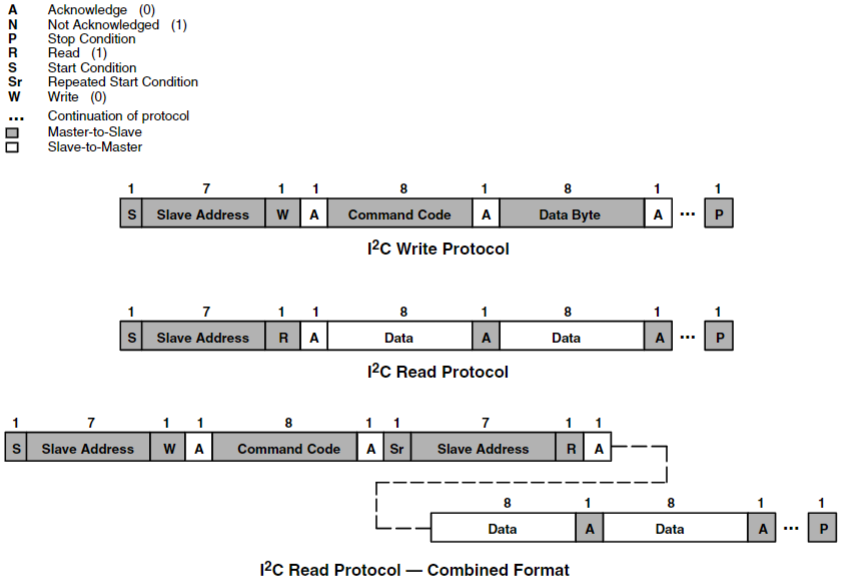
\includegraphics[width=\textwidth]{Immagini_sensore/I2C.png}
    \caption{I2C}
\end{figure}

La scrittura dei registri mediante I2C viene fatta mandando per prima cosa lo start bit, poi l'indirizzo della periferica e il write. Una volta ricevuto l'acknowledge si manda il Command code. Questo configura il registro di Command.

\begin{figure}
    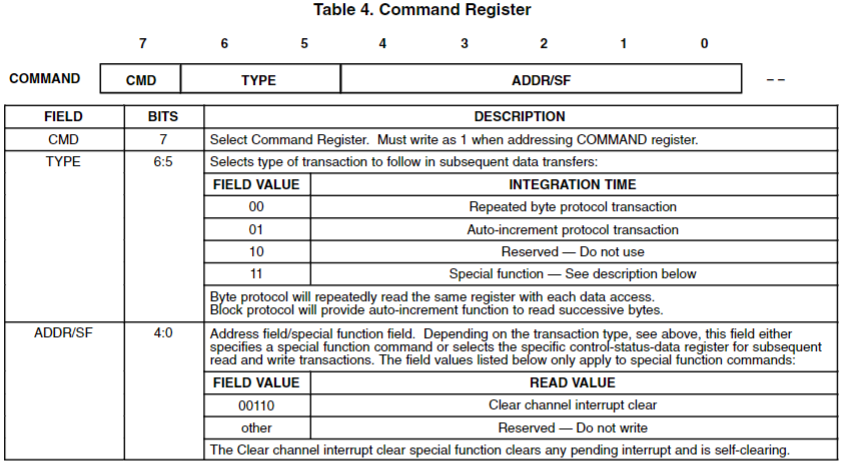
\includegraphics[width=\textwidth]{Immagini_sensore/registro_di_command.png}
    \caption{Registro Command}
    \label{fig:comm}
\end{figure}

Nel registro di Command possiamo stabilire se far leggere sempre lo stesso registro o scorrerli e da che indirizzo iniziare. Inoltre possiamo pulire gli interrupt.

Per la lettura, una volta impostato correttamente il registro command, basta mandare lo start, l'indirizzo e il read e lui continuerà dopo ogni ack a mandare il dato successivo fino a che non riceve lo stop bit.

\section{Macchina a Stati sensore}
\begin{figure}
    \centering
    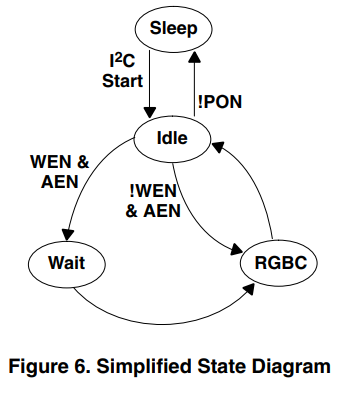
\includegraphics[width=0.4\textwidth]{Immagini_sensore/macchina_a_stati.png}
    \caption{Macchina a stati}
\end{figure}

Il sensore per risparmiare energia rimane nello stato di sleep. Una volta che riceve lo start dall'I2C va in idle ed in base a se è impostato il bit di wait o meno fa subito la misura oppure aspetta un certo tempo.

Una volta fatta la misura torna in idle e in caso di power on disabilitato torna in sleep. La macchina a stati dipende principalmente dai parametri del registro Enable (0x00).

\begin{figure}
    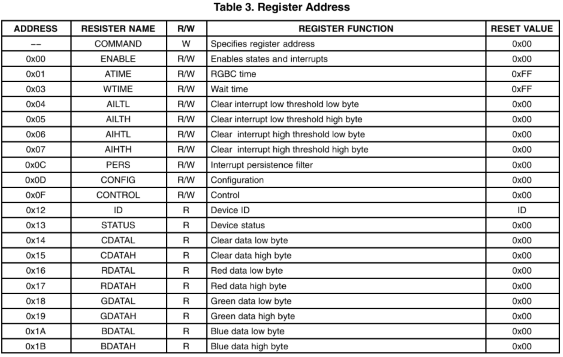
\includegraphics[width=\textwidth]{Immagini_sensore/Indirizzi_sensore.png}
    \caption{Registri sensore}
\end{figure} 

\section{Parametri scelti}
\label{sec:Parametri sensore}
\begin{table}
    \centering
    \begin{tabular}{ccc}
        Indirizzo & Nome & Valore \\
        ---- & Command & 10100000 \\
        0x00 & Enable & 0x03 \\
        0x01 & Timing & 0xC0 \\
        0x0F & Control & 0x03
    \end{tabular}
    \caption{Indirizzi settati}
    \label{tab:my_label}
\end{table}

Solo questi registri sono stati settati in quanto abbiamo scelto di non utilizzare l'interrupt per decidere quando leggere il sensore, ma piuttosto di fare un polling alla pressione di un pulsante ed eseguire a quel punto 3 misure così da implementare un voter.

Questo perché i livelli di luminosità registrati dal sensore erano simili tra con il cubetto sopra e senza e variavano più in base al colore del cubetto che dal fatto che fosse sopra o no.

\section{Command}
Come visibile nella figura \ref{fig:comm} per fare la lettura e scrittura abbiamo deciso di usare registro di Enable come primo registro e di fare le letture sequenziali degli indirizzi.

\section{Enable}

\begin{figure}
    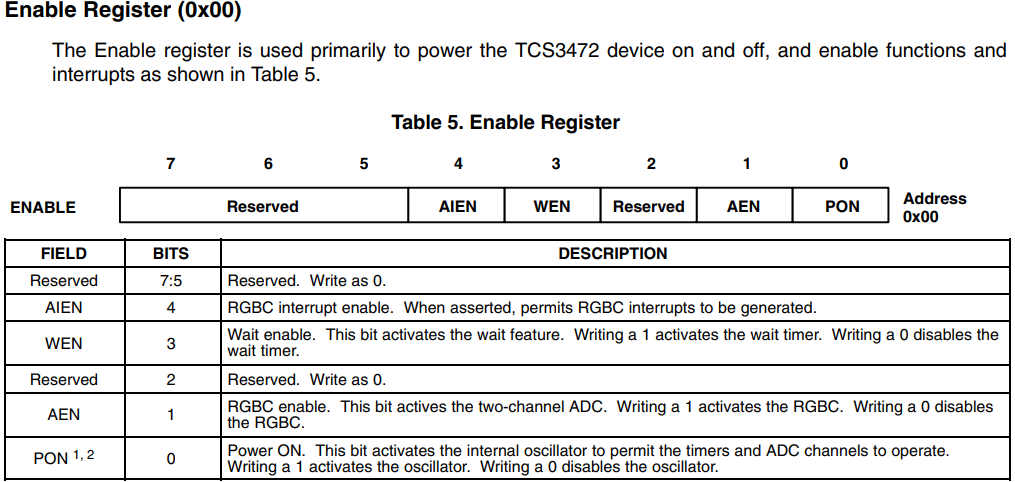
\includegraphics[width=\textwidth]{Immagini_sensore/registro_enable.png}
    \caption{Enable Register}
\end{figure}

Come scritto nella sezione \ref{sec:Parametri sensore} abbiamo ovviamente attivato il power on e gli ADC mentre non abbiamo attivato gli interrupt e il wait.

Non è stato attivato il wait in quanto per la nostra applicazione abbiamo preferito dare priorità alla velocità di lettura che al power management tenendo anche conto che si fanno 3 letture del sensore ogni volta.

\section{Timing e Control}
\begin{figure} 
    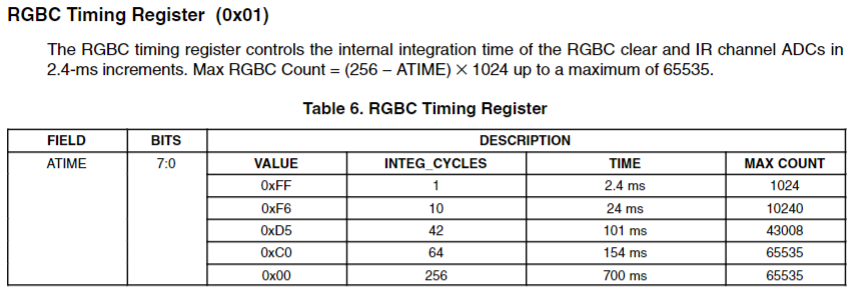
\includegraphics[width=\textwidth]{Immagini_sensore/registro_timing.png}
    \caption{Registro timing}
    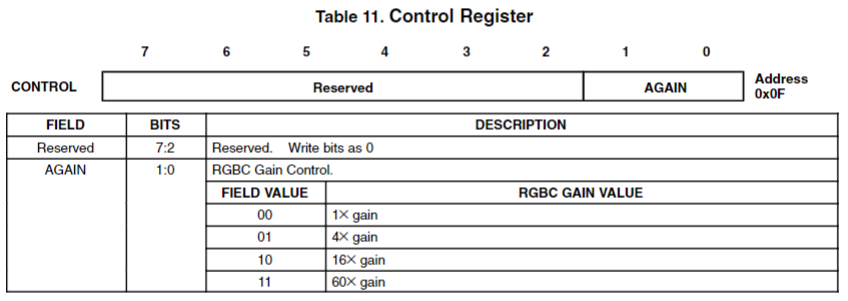
\includegraphics[width=\textwidth]{Immagini_sensore/registro_control.png}
    \caption{Registro control}
\end{figure}
    
I valori dei registri di timing e control sono stati scelti in tandem in quanto sono i valori che influenzano la lettura e la sua accuratezza. Il registro di timing modifica il tempo di integrazione degli ADC e quindi influisce sulla sensibilità e sulla risoluzione della misura mentre quello di control determina il guadagno dell'amplificatore.

Inizialmente per il timing ci siamo imposti un tempo massimo per le 3 misure di $1.5$ secondi. Sapendo che $Timing = (0xFF - 0xATIME) * 2.4ms$ Possiamo calcolare il \(ATIME_{min} = 0x2A\).

Abbiamo provato con il massimo guadagno (x60) e abbiamo aumentato il tempo di integrazione fino a raggiungere dei valori con un buon valore massimo e minimo con tutti i colori evitando la saturazione ovvero \(ATIME_{1} = 0xC0\) ovvero Timing = $154ms$ così da avere un buon compromesso tra il tempo di integrazione e la risoluzione e sensibilità dei valori misurati.

 Successivamente abbiamo fatto una prova usando il massimo tempo di integrazione considerato accettabile (\(ATIME_{2} = 0x2A\)  ovvero Timing = $510ms$) ed aumentato il guadagno fino ad arrivare ad un valore né troppo basso né in saturazione per ogni colore, ovvero (x16).
    
\label{sec:Timing}
    \begin{table}
        \centering
        \begin{tabular}{ccc}
            Registro & Configurazione 1 & Configurazione 2\\
             Timing& 0xC0 & 0x2A\\
             Control& 0x03 & 0x02\\
        \end{tabular}
        \caption{Configurazioni}
        \label{tab:configurazioni}
    \end{table}
    
    \begin{table}
        \centering
        \begin{tabular}{ccc}
            Registro & Configurazione 1 & Configurazione 2\\
             $Red_L$& 01 & 6A\\
             $Red_H$& FF & D6\\
             $Green_L$& 31 & E4\\
             $Green_H$& 2F & 26\\
             $Blue_L$& 62 & 97\\
             $Blue_H$& 25 & 1F\\
        \end{tabular}
        \caption{Cubo rosso}
        \label{tab:cubo_rosso}
    \end{table}
    
    \begin{table}
        \centering
        \begin{tabular}{ccc}
            Registro & Configurazione 1 & Configurazione 2\\
             $Red_L$& 2D & E4\\
             $Red_H$& 49 & 43\\
             $Green_L$& 03 & 2B\\
             $Green_H$& 80 & 79\\
             $Blue_L$& 77 & F4\\
             $Blue_H$& 6C & 66
        \end{tabular}
        \caption{Cubo blu}
        \label{tab:cubo_blu}
    \end{table}
        
    \begin{table}
        \centering
        \begin{tabular}{ccc}
            Registro & Configurazione 1 & Configurazione 2\\
             $Red_L$& 79 & 48\\
             $Red_H$& 5A & 55\\
             $Green_L$& CD & 89\\
             $Green_H$& 80 & 7C\\
             $Blue_L$& 9A & 6C\\
             $Blue_H$& 3D & 38
        \end{tabular}
        \caption{Cubo verde}
        \label{tab:cubo_verde}
    \end{table}
    
Vedendo che la differenza tra le due configurazioni era trascurabile, si è optato per l'uso della prima, così da risparmiare un secondo nella misura.

Un problema riscontrato è stato quello della misura sul cubo blu in quanto il colore dal valore più alto è risultato il verde ed il blu solo il secondo più alto. Provando a cambiare colore con un cartoncino più scuro il colore con il valore più alto risultava invece il rosso a causa del grande assorbimento di luce del cartoncino blu scuro. Questo è dovuto in parte al fatto che la luce del led in dotazione tende un po' verso il giallo (componente rossa più accentuata) e alla maggior responsività alla luce rossa e verde rispetto alla blu.

\section{Lettura}

\begin{figure}
    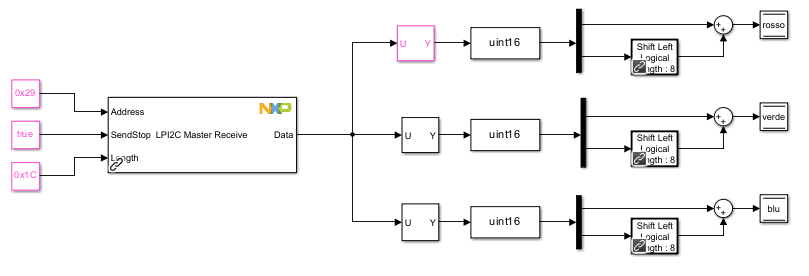
\includegraphics[width=\textwidth]{Immagini_sensore/lettura_sensore.png}
    \caption{Lettura sensore}
    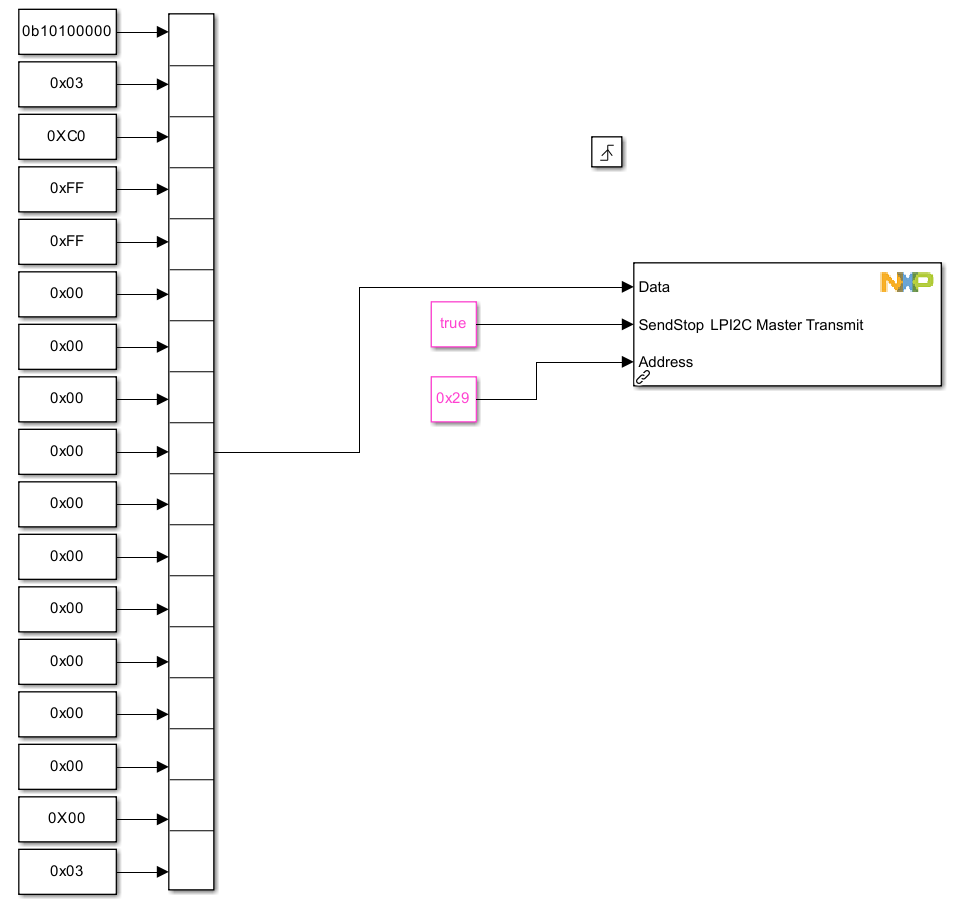
\includegraphics[width=0.4\textwidth]{Immagini_sensore/scrittura_sensore.png}
    \caption{Scrittura sensore}
\end{figure}

Si è deciso di leggere tutti i blocchi ogni volta che fosse stata necessaria la lettura, per evitare dopo la scrittura di dover riscrivere il registro command con il nuovo indirizzo di partenza, visto che il guadagno in termini di tempo era trascurabile.

Una volta eseguita la lettura di esegue la somma pesata dei valori H e L dei registri di ogni colore per avere il valore effettivo a 16 bit.

\section{Macchina a stati}
\begin{figure}

    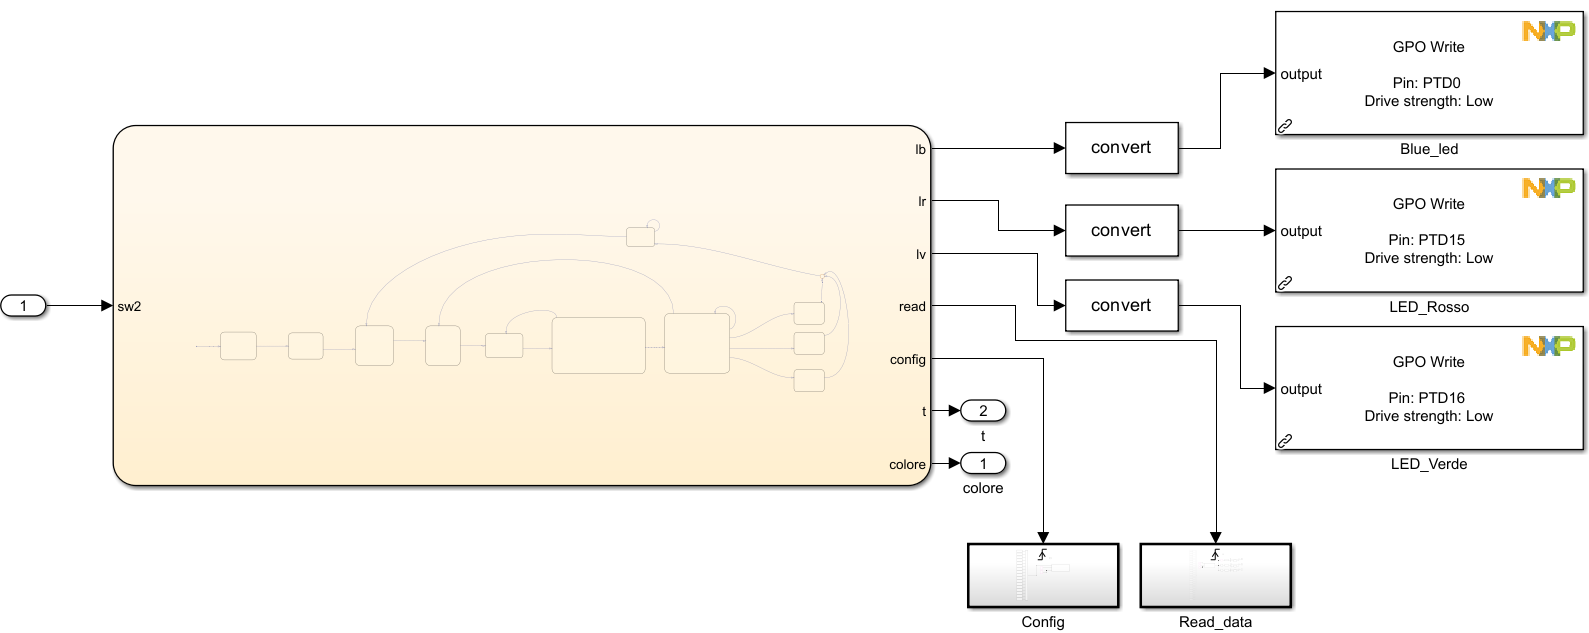
\includegraphics[width=\textwidth]{Immagini_sensore/Sensing_e_macchina_a_stati.png}
    \caption{Matlab sensing}
    \end{figure}
    
\begin{figure}
    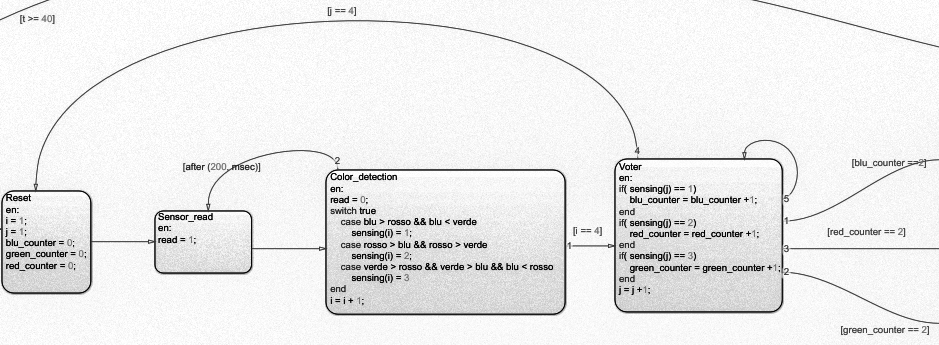
\includegraphics[width=\textwidth]{Immagini_sensore/sensor_chart.png}
    \caption{Macchina a stati}
    \label{fig:stateflow}
\end{figure}

Come possiamo vedere nella figura \ref{fig:stateflow}, all'accensione viene configurato il sensore e messo colore a 4 per mettere il braccio in una posizione di default.

Successivamente si entra in uno stato di wait in cui si resettano tutti i contatori.

Premendo il pulsante sw2 si passa allo stato di reset del voter.

Si eseguono 3 letture con conseguente decisione del colore per ogni misura. A quel punto il voter decide il colore del cubo se vi sono 2 colori uguali oppure rifà le misure se sono tutti e 3 diversi.

Per finire incrementa un contatore ogni 200ms per temporizzare l'attuazione.

\section{Voter}

\begin{figure}
    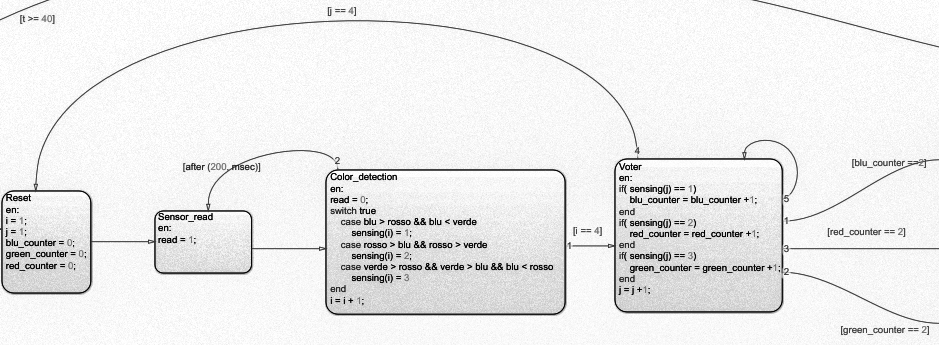
\includegraphics[width=\textwidth]{Immagini_sensore/voter.png}
    \caption{Voter}
\end{figure}

Per stabilire con accuratezza il colore del cubo è stato necessario implementare un voter in quanto durante i test la misura a volte risultava diversa.

Per cui abbiamo deciso di applicare una ridondanza nelle misure a scapito della velocità di misura.

Per le ragioni esposte nella sezione \ref{sec:Timing}, nel blocco \textbf{color detection} è stato necessario, per il riconoscimento del blu, mettere i valori del blu compresi tra la soglia del verde e la soglia del rosso.

\section{Test}

Purtroppo non è stato possibile fare il PIL dei blocchi contenenti la comunicazione via I2C, in quanto incompatibili.

\begin{figure}
    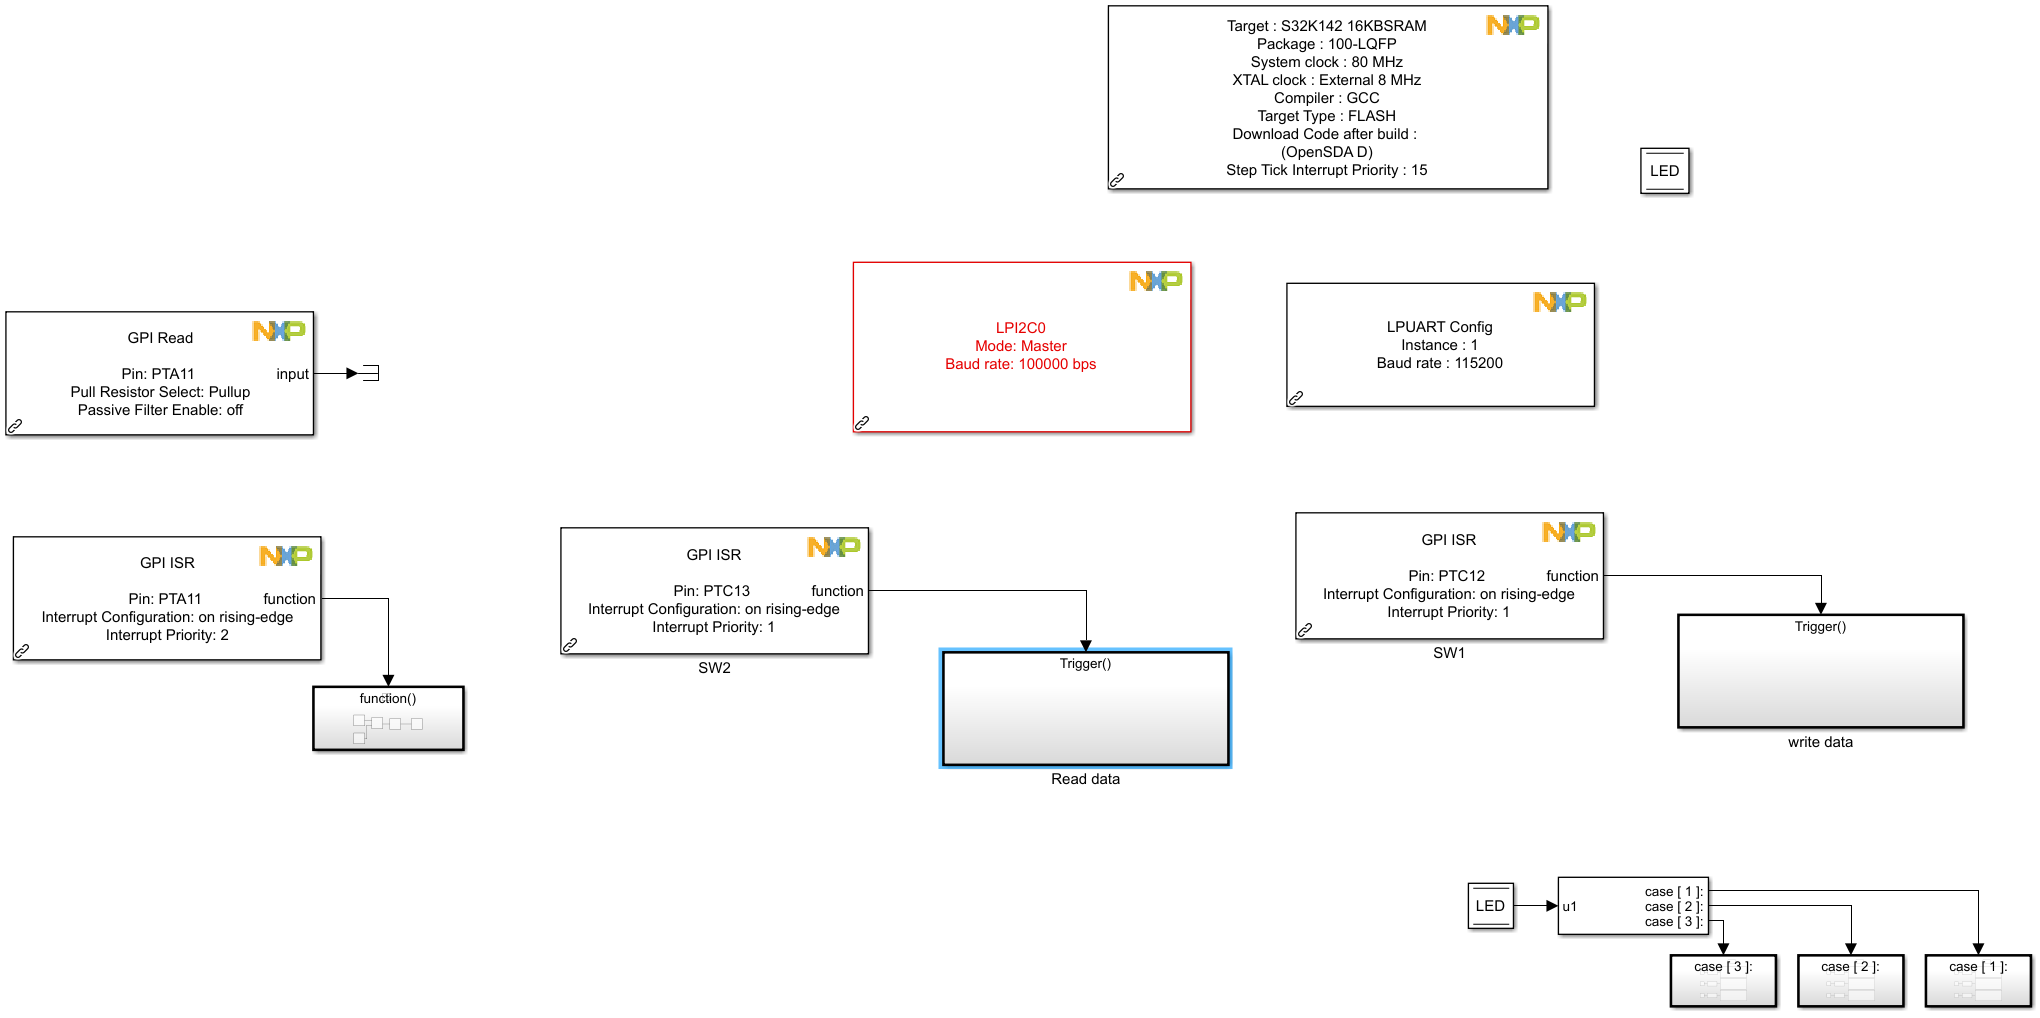
\includegraphics[width=\textwidth]{Immagini_sensore/i2c_test.png}
    \caption{Test I2C}
\end{figure}

Per eseguire i test della parte di sensore, inizialmente è stato fatto un file Matlab che si occupava solo di comunicare con il sensore e mandare i dati ricevuti via uart al pc così da poter valutare i parametri migliori per il sensore.

Una volta individuati è stata fatta la macchina a stati e testata prima in MIL e poi usando la uart e il led rgb per il debug.

\begin{figure}
    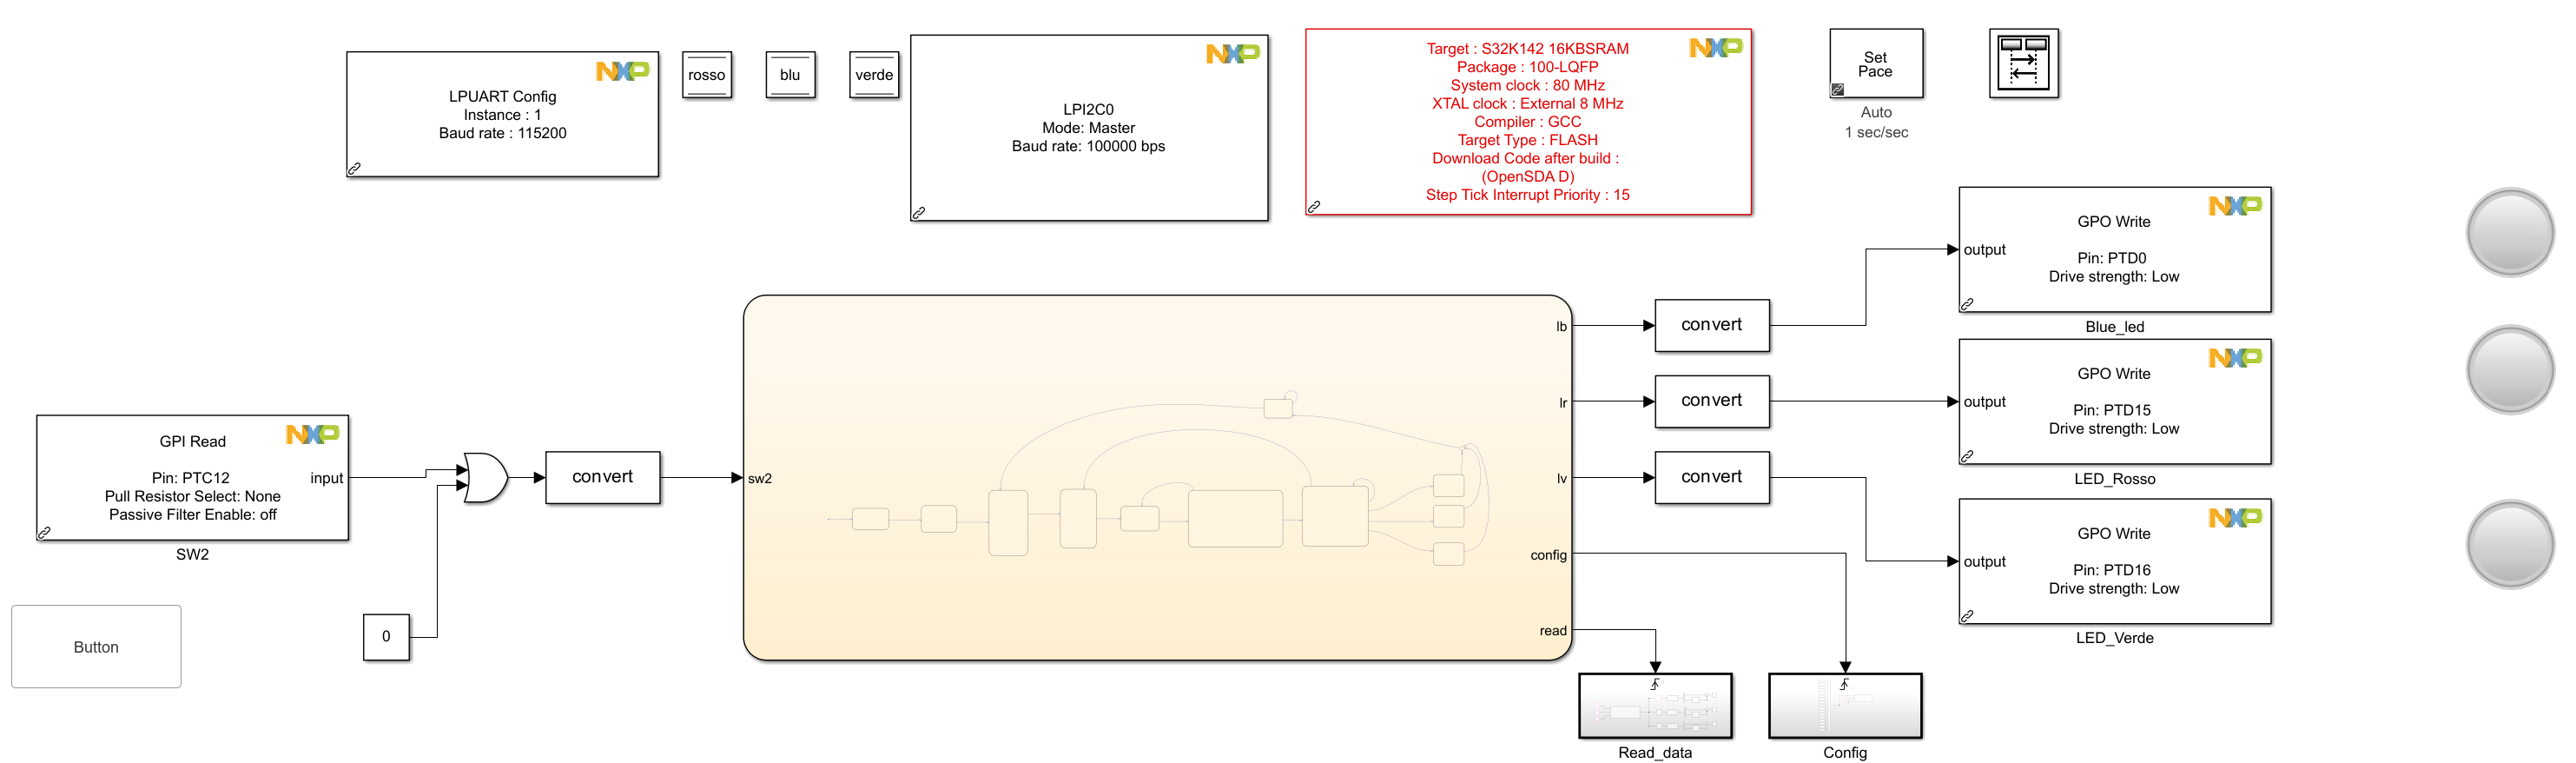
\includegraphics[width=\textwidth]{Immagini_sensore/test_stateflow_2.png}
    \caption{Test macchina a stati}
\end{figure}

\begin{figure}[h] 
    \centering
    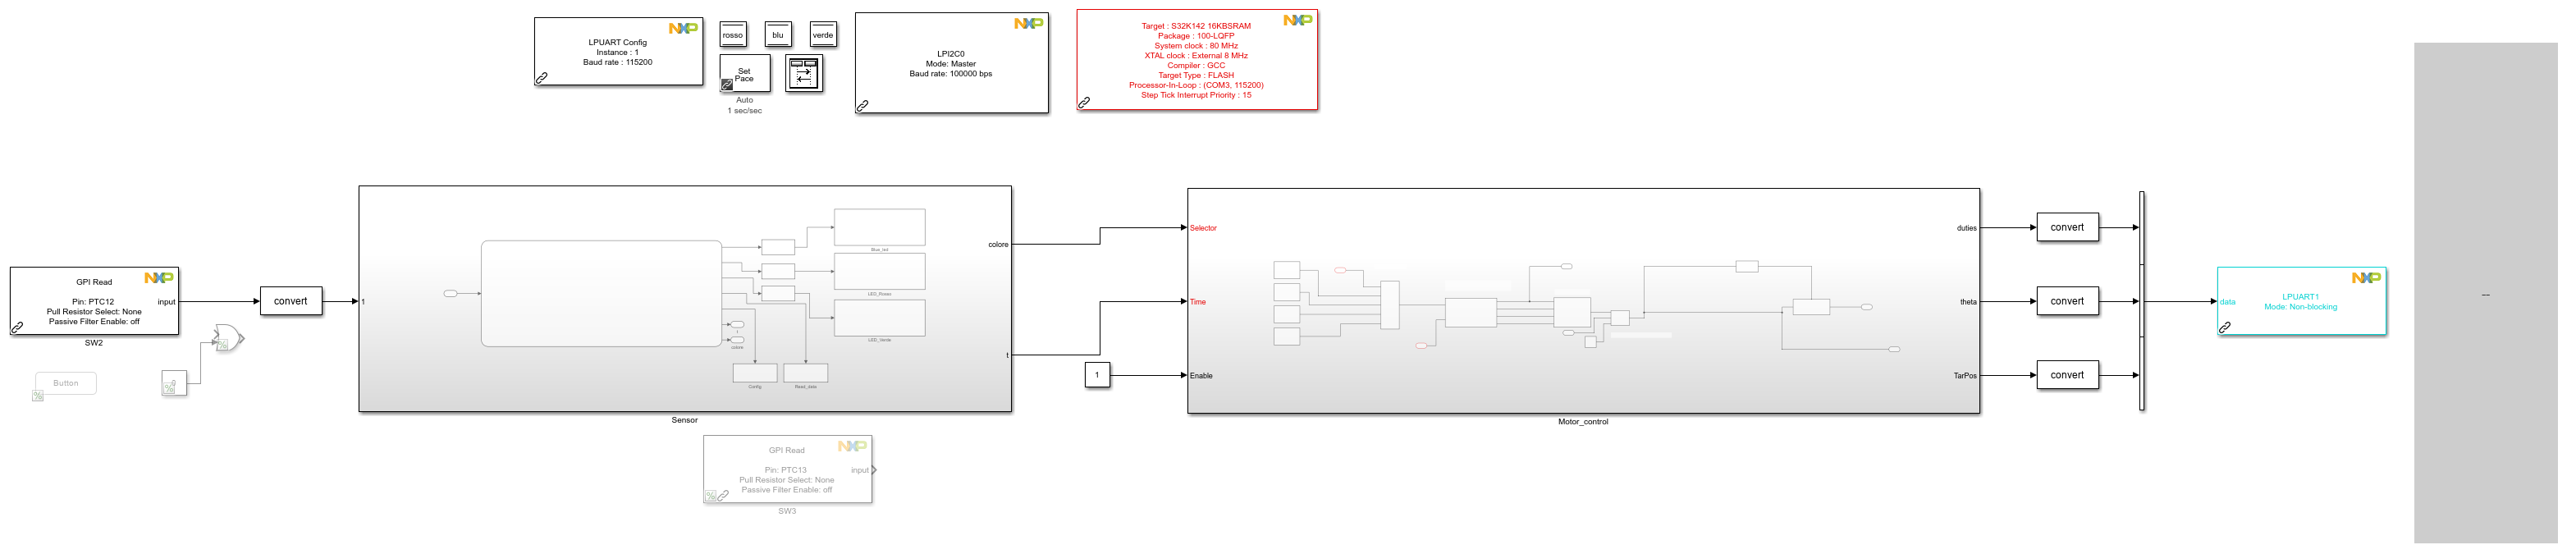
\includegraphics[width=\textwidth]{Immagini_sensore/Matlab_completo.png}
    \caption{MIL completo}
\end{figure}

\chapter{Attuazione}

Il modulo di attuazione controlla l'uscita PWM per i servo-motori per guidare il braccio robotico lungo percorsi predefiniti.

Due input determinano il percorso da seguire e il punto corrente del percorso.

Altri input e output sono usati solo in fase di debug.

Il modulo è stato ideato per permettere un controllo semplice della velocità di esecuzione e flessibilità nella scelta del percorso.

\section{Principio di funzionamento}

\begin{figure}
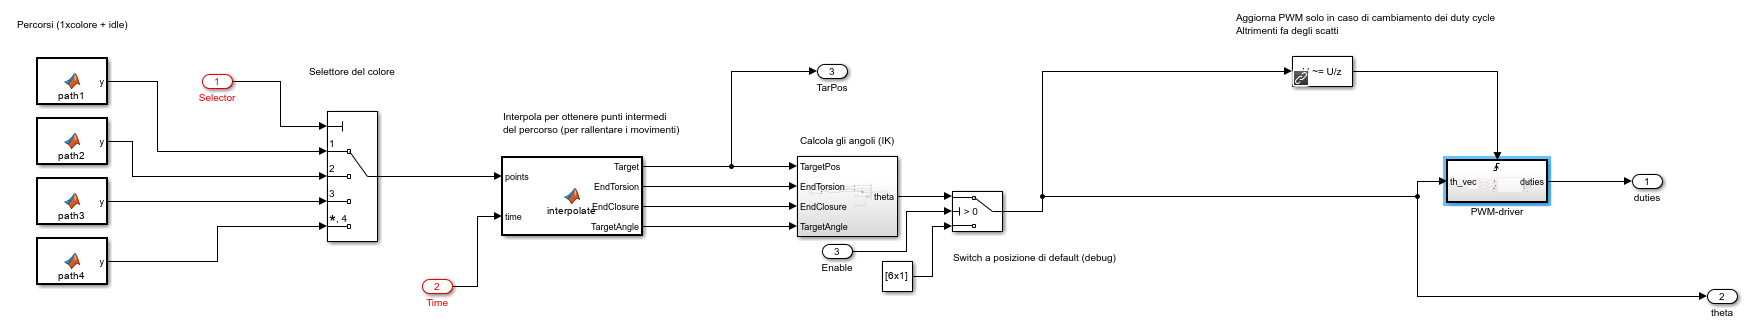
\includegraphics[width=\textwidth]{Complete_attuation}
\caption{Diagramma completo}
\end{figure}

I blocchi \textbf{Path1...Path4} restituiscono ognuno una matrice costante che rappresenta un percorso per il braccio robotico. Ogni riga rappresenta un punto chiave del percorso. A partire dai punti chiave vengono successivamete calcolati punti intermedi.

Ogni riga contiene 7 elementi:

\begin{itemize}
\item Distanza radiale in coordinate cilindriche dell'obiettivo dal centro della base del braccio robotico.
\item Angolo in cordinate cilindriche dell'obiettivo.
\item Distanza verticale in coordinate cilindriche dell'obiettivo dalla base del braccio robotico.
\item Angolo tra il vettore parallelo all'ultimo segmento del manipolatore (positivo verso la pinza) e la verticale (positiva verso l'alto).
\item Angolo del polso.
\item Angolo di chiusura della pinza.
\item Istante temporale del punto nel percorso.
\end{itemize}

\begin{figure}
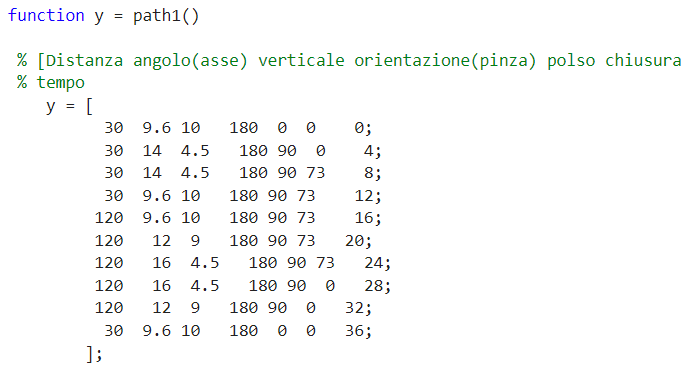
\includegraphics[width=\textwidth]{Path_structure}
\caption{Esempio di percorso}
\end{figure}

L'input \textbf{Selector} determina quale percorso verrà usato.

Il blocco \textbf{Interpolate} genera un punto intermedio interpolando linearmente due punti successivi nel percorso in base all'input \textbf{Time}.

Parte del blocco serve a garantire le corrette dimensioni della matrice in ingresso.

Vengono usati i punti estremi se \textbf{Time} eccede gli istanti temporali estremi.

Il blocco successivo calcola gli angoli dei servo-motori a partire dal punto interpolato.

Lo switch che segue permette di sostituire gli angoli calcolati con angoli predefiniti, per portare il manipolatore in una configurazione sicura durante il debug.

Il blocco \textbf{PWM-driver} imposta le uscite PWM a partire dagli angoli desiderati.

Questo blocco viene eseguito solo se gli angoli desiderati cambiano.

\section{Reimpostazione periodica del PWM}

Se il blocco \textbf{PWM-driver} venisse attivato liberamente (senza trigger al cambiamento) i servo-motori subirebbero uno scatto dovuto alla reimpostazione del PWM, che avviene anche quando i duty-cycle non variano.

Per questo è importante usare il blocco \textbf{Detect Change}. 

\section{Cinematica inversa}

Ci sono 6 motori in totale, denominati da M1 a M6.

M6 controlla la chiusura della pinza, M5 la rotazione del polso. I motori che determinano posizione e orientazione dell'end-effector sono 4.

M2, M3 e M4 possono spostare l'end-effector solo sul piano determinato da M1. Fissata la posizione dell'end-effector, è determinata la rotazione di M1 per avere l'allineamento. Fissata anche l'orientazione finale desiderata, anche la posizione di M4 è identificata. Data questa, M2 e M3 formano uno Scara con M4 come end-effector.

\section{Test}

Il sistema di attuazione è stato prima verificato in SIL e in PIL in più iterazioni.

Sono stati progressivamente aggiunti blocchi ad ogni iterazione che ha avuto successo, in questo ordine: PWM-driver, IK, Interpolate, Selector.

Le uscite di debug mostrano la posizione desiderata, gli angoli previsti e i duty cycle impostati.

Un input di debug permette di riportare il braccio in una posizione sicura ed è stato usato in PIL.

\begin{figure}
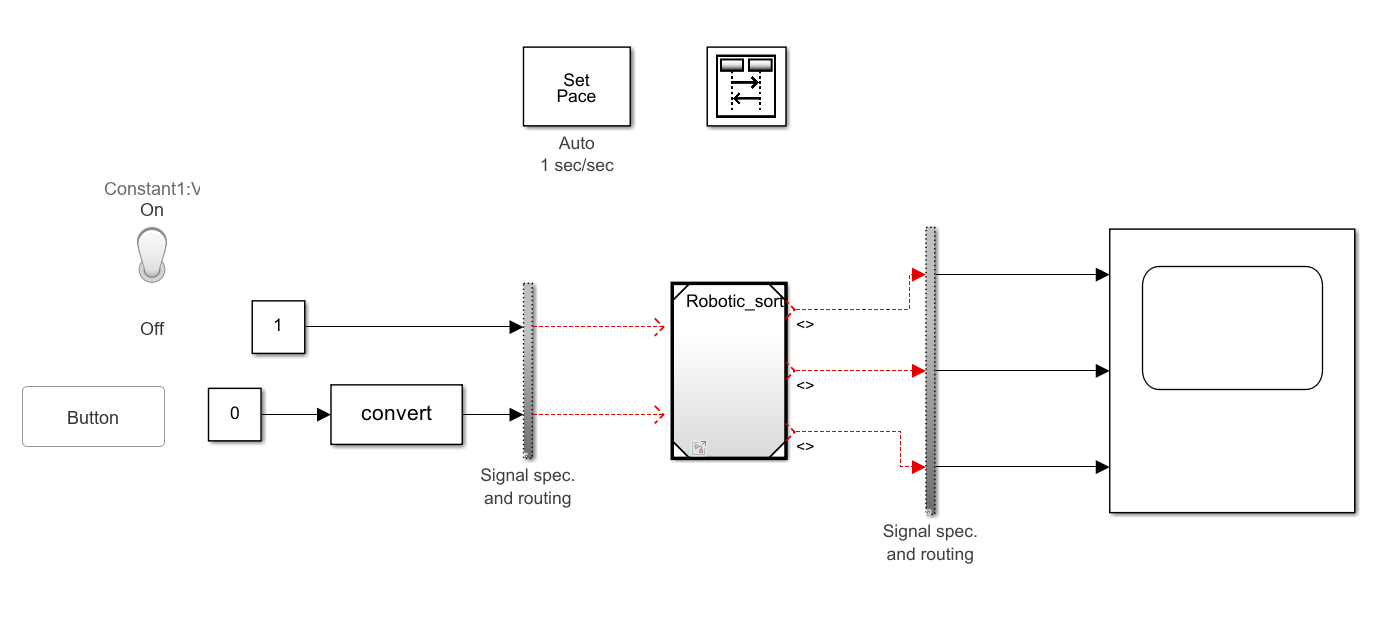
\includegraphics[width=\textwidth]{Harness}
\caption{Harness del modulo di attuazione (screenshot scattato a fine progetto, differisce parzialmente da quello usato).}
\end{figure}

\chapter{Verifica finale}

\begin{figure}[h] 
    \centering
    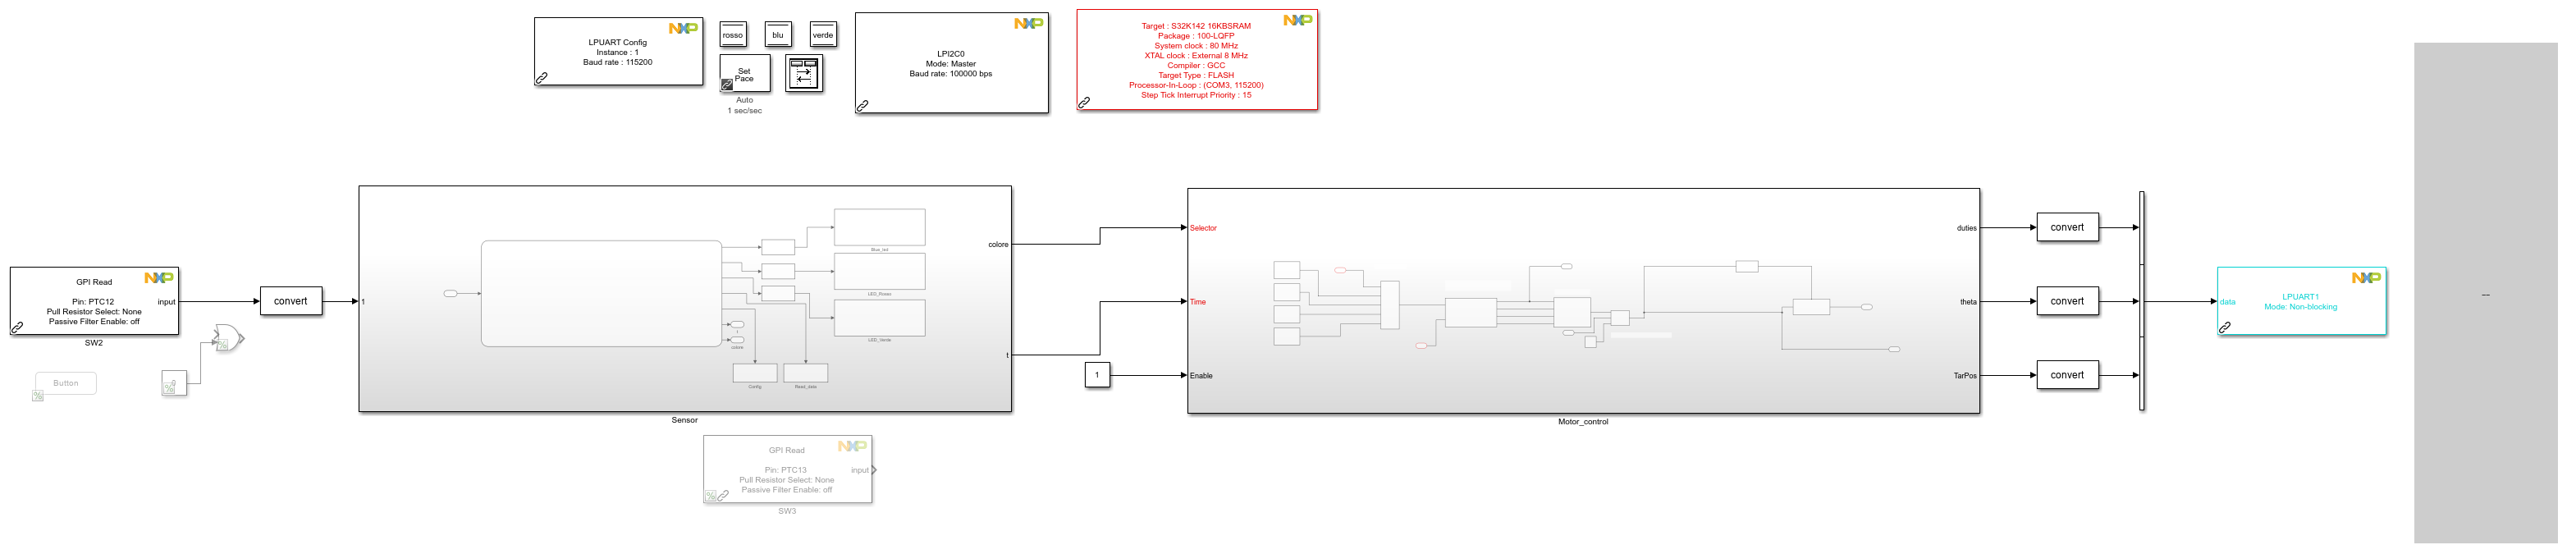
\includegraphics[width=0.75\textwidth]{Immagini_sensore/Matlab_completo.png}
    \caption{MIL completo}
\end{figure}

Sviluppati e verificati indipendentemente i due moduli, abbiamo cominciato la fase finale.

I due moduli sono stati combinati velocemente, grazie alla semplice interfaccia.

Ci siamo accorti di non poter fare simulazioni \emph{in the loop} perché incompatibili con la periferica I2C.

Abbiamo usato la UART per verificare che tutto proseguisse come previsto durante la verifica.

Non abbiamo riscontrato problemi oltre all'impossibilità di usare SIL/PIL o i timer (per mandare messaggi temporizzati tramite UART). Così abbiamo subito potuto definire e verificare i percorsi.

Avevamo preparato delle bozze dei percorsi usando un modello del braccio realizzato e animato su Blender3D. Modificando queste in base alle verifiche abbiamo ottenuto dei percorsi che ci soddisfacessero.

\begin{figure}
\centering
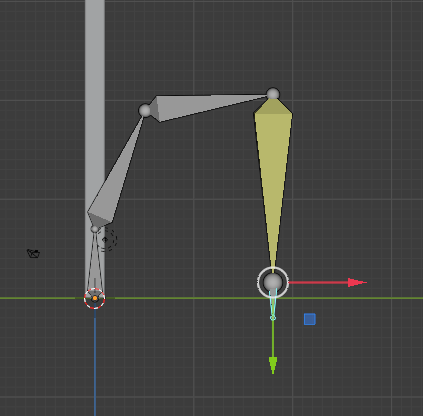
\includegraphics[width=0.4\textwidth]{Blender3D}
\caption{Armatura del braccio su Blender3D}
\end{figure}

\chapter{Problemi durante lo sviluppo}

Durante i test PIL, due pezzi stampati 3D per la trasmissione della coppia da servo-motori a struttura si sono rotti. In particolare si sono spanati gli incastri per i servo-motori.

Il primo guasto è stato dovuto a un blocca di ritardo nell'harness: la condizione iniziale ha fatto piegare il braccio su se stesso all'avvio.

Il secondo guasto è stato dovuto alla base fissata male (svitando le viti si sono rovinati i fori) in seguito alle riparazioni del guasto precedente.

Altri problemi sono stati riscontrati durante la fase di test del sensore, in quanto risultava difficoltoso trovare un materiale che non fosse troppo assorbente o riflettente e un blu non fosse troppo scuro o troppo chiaro così da poter distinguerlo in modo affidabile dagli altri colori.

\chapter{Conclusione}

Realizzata la parte funzionale, abbiamo preparato una base pieghevole su cui abbiamo montato la pedana di riconoscimento e dei cartoncini colorati per indicare le zone di smistamento.

Riguardo la parte di attuazione, i due passaggi chiave sono stati la riduzione dell'algoritmo IK a quello di uno scara e l'uso estensivo di SIL e PIL.

Mentre per quanto riguarda la fase di percezione i passaggi chiave sono stati la scelta dei parametri del sensore con la scelta dei colori e finiture migliori dei cubi colorati, l'uso della UART per il debug e l'interpretazione di un voter.

Noi possiamo ritenere con soddisfazione questo progetto un successo, dal punto di vista sia del risultato finale, sia della flessibilità e futura modificabilità della funzione, sia del processo in sé.

\end{document}